%\section{Stability Control}
\section{Mechanisms of Trajectory Stability Under the Signal-Interference Framework}

The sample-level quantities $S_1$, $S_2$, and $S_3$ used in these results are defined in Appendix~\ref{appendix:sample-level}, with the iteration indexing used by the experiments below.

In modern deep learning, training stability is typically achieved through a set of standard heuristics, like momentum~\cite{polyak1964methods,smith2018disciplined}, weight decay~\cite{krogh1991simple,loshchilov2017decoupled}, learning-rate schedules~\cite{smith2017cyclical,loshchilov2016sgdr}, adaptive methods such as Adam~\cite{kingma2014adam}, and more recently gradient orthogonalization~\cite{jordan2024muon}. Here we argue that these methods can be viewed as explicit mechanisms for controlling the signal--interference trade-off: they either promote constructive accumulation ($S_1+S_2$) or mitigate destructive cross-step interference ($S_3$) by reshaping the magnitude, direction, and temporal structure of the updates.

In this section, we focus on plain SGD, momentum, and weight decay, as they provide the foundational building blocks for adaptive optimization and regularization, which are central to deep learning stability and scale. We first analyze SGD trajectories using the diagnostic in Eq.~\eqref{eq:rho} and identify three regimes: an early constructive phase ($\rho_t>0$), a destructive phase ($\rho_t<0$), and a final random drift phase ($\rho_t\approx 0$). We then examine momentum and weight decay, interpreting how each affects the signal--interference trade-off. Next, we run ablations using plain SGD, SGD with momentum, and SGD with weight decay. Finally, we show how batch representativeness explains the coherence and stability of SGD. We follow the benchmark setting used in the Edge-of-Stability literature~\cite{cohen2021edge}, training VGG~\cite{simonyan2014vgg} on CIFAR-10~\cite{krizhevsky2009cifar}.

%\subsection{SGD Learning Phases}
\subsection{Trajectory Regimes in Plain SGD}

Here we analyze training dynamics of plain SGD using the consecutive-gradient cosine diagnostic introduced in Eq.~\eqref{eq:rho}. We trained using plain SGD for a fixed number of iterations ($T = 100{,}000$), varying the batch size over \(m \in \{8,32,128,512\}\) while keeping the learning rate fixed at \(\eta = 0.01\). Figure~\ref{fig:cifar_traj} shows the smoothed evolution of the training loss, parameter norm, gradient norm, and cosine similarity between successive mini-batch gradients. Because both \(T\) and the dataset size \(N\) are fixed, larger batch sizes correspond to a larger number of training epochs. Therefore, differences across \(m\) reflect both changes in gradient stochasticity and changes in the total amount of data processed during training. %Because both \(T\) and the dataset size \(N\) are fixed, larger batch sizes correspond to a larger number of effective training epochs.

\begin{figure*}
    \centering
    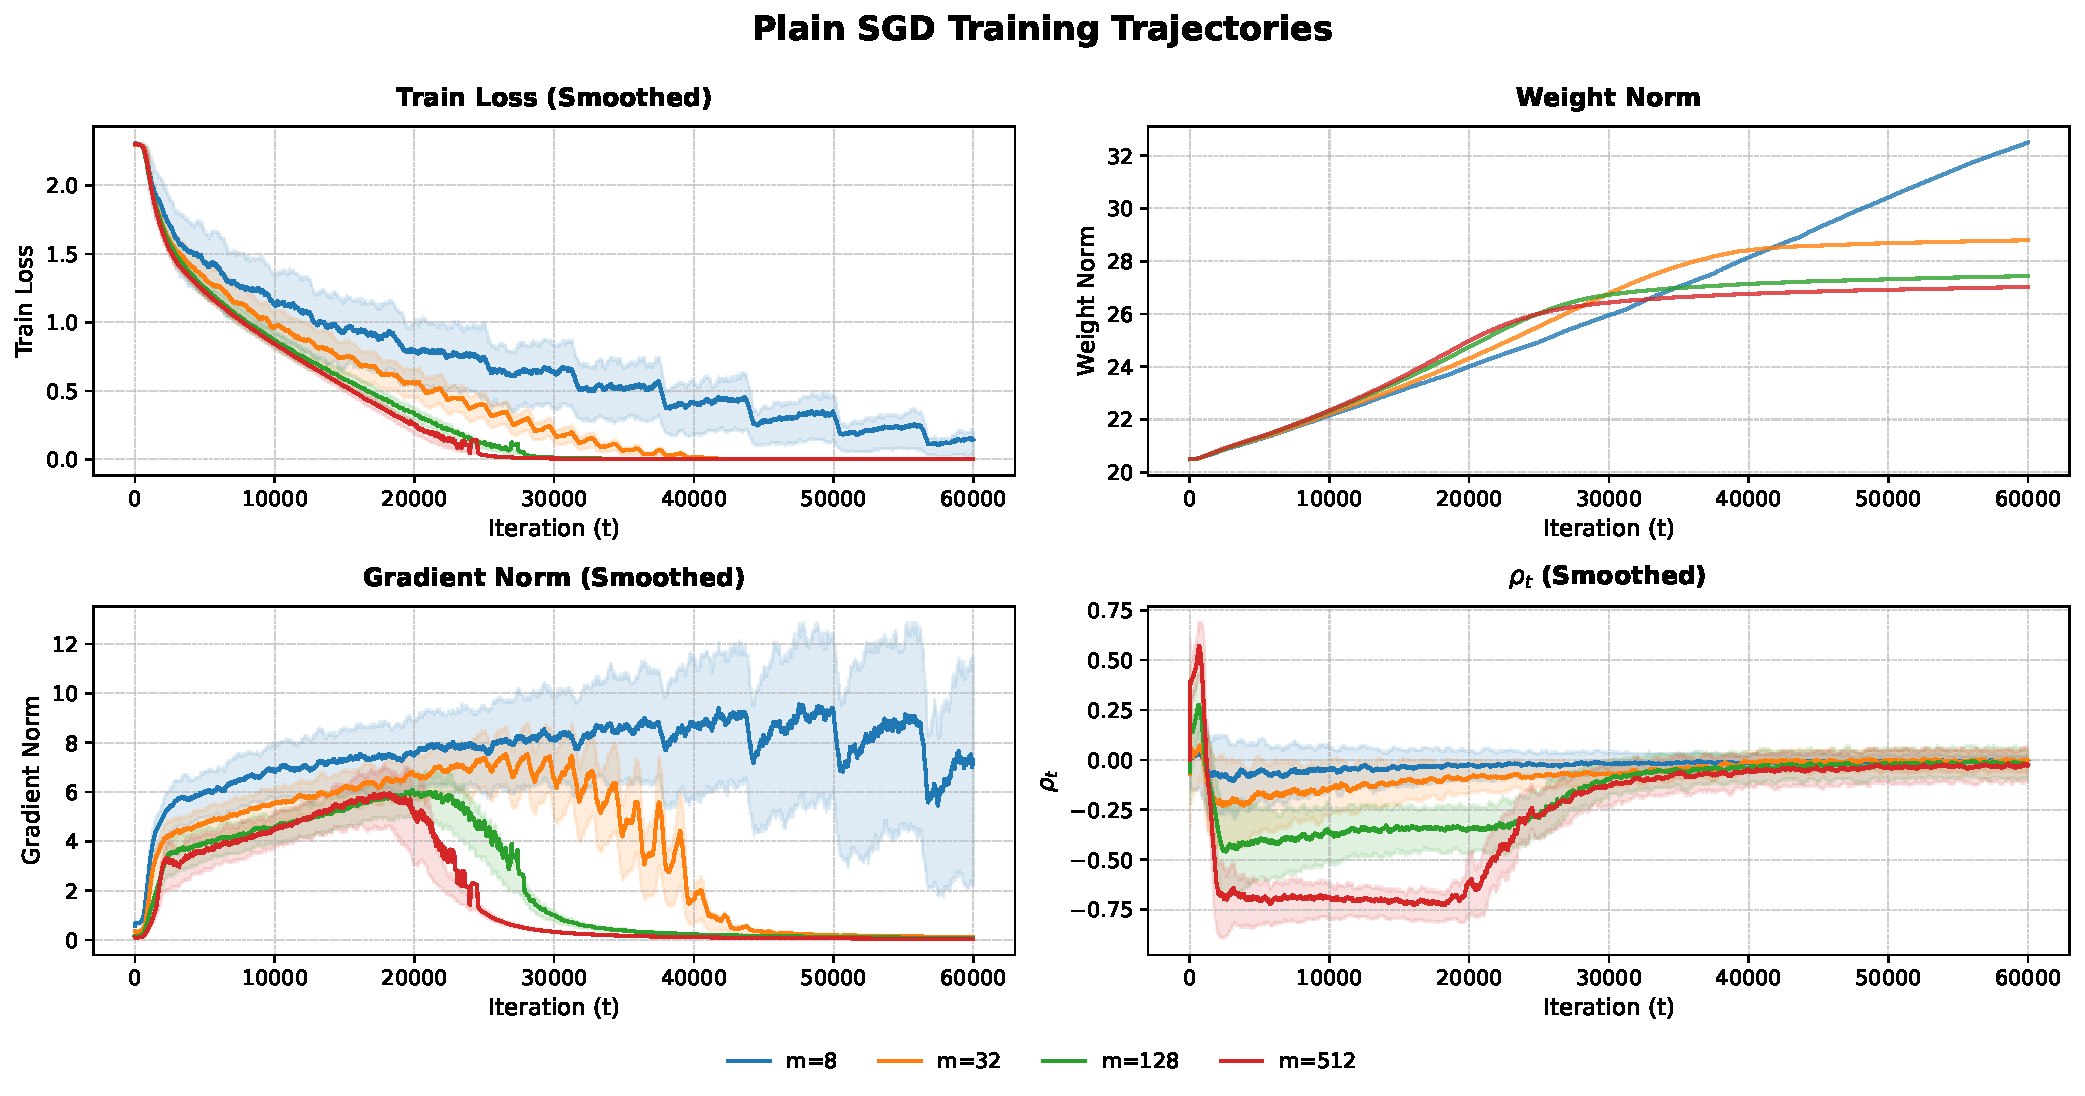
\includegraphics[width=1\linewidth]{figures/traj_metrics_cifar10_less_batches.pdf}
    \caption{Smoothed training trajectories for plain SGD with $\eta = 0.01$. The plot grid shows training loss, the model's weight norm, gradient norms, and the cosine similarity between the gradients of sequential batches.}
    \label{fig:cifar_traj}
\end{figure*}


Across all batch sizes, the training trajectories follow a consistent three-phase pattern. In the initial phase, successive gradients are strongly aligned, as indicated by positive cosine similarity, as shown in the bottom-right corner plot of Fig. \ref{fig:cifar_traj}. This alignment is stronger for larger batches and corresponds to rapid loss reduction and steady growth of the parameter norm, reflecting effective accumulation of the learning signal. As training progresses, an oscillatory phase emerges in which cosine similarity becomes negative. This indicates that successive updates partially oppose one another, consistent with overshooting and oscillation around a minimum. In the final phase, cosine similarity approaches zero, indicating that successive gradients are largely uncorrelated. In this regime, loss improvement saturates, and training becomes noise-dominated: parameter updates behave like a random walk, and further norm growth is driven primarily by stochastic fluctuations rather than a consistent learning signal.

Training dynamics vary systematically with batch size. For larger batches, the three phases are clearly separated, and the optimization trajectory is well structured. Gradient estimates are more accurate, leading to strong early alignment, a clear oscillatory phase near the minimum, and eventual convergence. As the batch size decreases, the magnitude of $\rho_t$ decreases, indicating weaker gradient alignment and larger stochasticity. For the smallest batch size (\(m = 8\)), training is largely noise-dominated: the loss and gradient norms fluctuate strongly, while the parameter norm continues to grow. In this regime, weight growth is driven primarily by stochastic noise rather than by a consistent learning signal, indicating that noise is being absorbed into the parameters without stable convergence.

%\subsection{Momentum}
\subsection{Momentum as Temporal Averaging}
\label{subsec:momentum_method}

Plain SGD exhibits an oscillatory regime in which consecutive updates partially cancel each other, leading to negative cross-step interference ($S_3<0$). Momentum mitigates this behavior by averaging gradients over time, thereby smoothing the trajectory and promoting more consistent update directions. Here, we consider SGD with momentum~\cite{polyak1964methods}. Let $\mu\in[0,1]$ be the momentum coefficient and $p_t\in\mathbb{R}^d$ the velocity, with $p_0=0$. The updates are

\begin{equation}
\label{eq:momentum_updates}
\begin{aligned}
  p_{t+1} &= \mu p_t + G_{B_t}(\theta_t),\\
  \theta_{t+1} &= \theta_t - \eta\, p_{t+1}.
\end{aligned}
\end{equation}
%with $G_{B_t}(\theta_t)=\frac{1}{m}\sum_{i=1}^m g_i^{(t)}$ and $g_i^{(t)}=\nabla_\theta\ell(\theta_t;x_i,y_i)$. 
Unrolling the recursion yields $p_{t+1}=\sum_{u=0}^{t}\mu^{t-u}G_{B_u}(\theta_u)$, and telescoping $\theta_{t+1}-\theta_t=-\eta p_{t+1}$ gives
\begin{equation}
\begin{aligned}
\label{eq:thetaT_momentum}
\theta_T
&=\theta_0-\eta\sum_{t=0}^{T-1}\alpha_t\,G_{B_t}(\theta_t),
\\
\alpha_t
&:=\sum_{r=0}^{T-1-t}\mu^r
=
\frac{1-\mu^{T-t}}{1-\mu}.
\end{aligned}
\end{equation}
%
Expanding the squared norm as in Eq.~\eqref{eq:s_def}, we obtain the momentum-weighted trade-off decomposition
\begin{equation}
\label{eq:thetaT_full_momentum}
\|\theta_T\|^{2}
=\|\theta_0\|^{2}
+ C^{(\mu)}
+\frac{\eta^{2}}{m^{2}}\bigl(S_1^{(\mu)}+S_2^{(\mu)}+S_3^{(\mu)}\bigr),
\end{equation}
where
\begin{align}
C^{(\mu)}
&:=
-2\frac{\eta}{m}\sum_{t=0}^{T-1}\sum_{i=1}^{m}\alpha_t\,\theta_0^{\top}g_i^{(t)},
\label{eq:C_mu}\\
S_1^{(\mu)}
&:=
\sum_{t=0}^{T-1}\alpha_t^2\sum_{i=1}^{m}\|g_i^{(t)}\|^2,
\label{eq:S1_mu}\\
S_2^{(\mu)}
&:=
\sum_{t=0}^{T-1}\alpha_t^2\sum_{i=1}^{m}\sum_{\substack{j=1\\ j\neq i}}^{m} g_i^{(t)\top}g_j^{(t)},
\label{eq:S2_mu}\\
S_3^{(\mu)}
&:=
2\sum_{t=0}^{T-1}\sum_{u=0}^{t-1}\alpha_t\alpha_u\sum_{i=1}^{m}\sum_{j=1}^{m} g_i^{(t)\top}g_j^{(u)}.
\label{eq:S3_mu}
\end{align}
%
From Eqs.~\eqref{eq:thetaT_momentum}--\eqref{eq:S3_mu}, momentum can be interpreted as a temporal averaging mechanism. Because each update direction \(p_{t+1}\) is an exponentially weighted average of recent mini-batch gradients, momentum smooths high-frequency batch-to-batch variation and tends to make successive updates more coherent. In the signal--interference decomposition, this typically reduces destructive cross-step cancellation and can shift the trajectory toward more constructive accumulation (\(S_3 > 0\)). At the same time, the coefficients \(\alpha_t\) show that earlier gradients have a larger cumulative influence on \(\theta_T\), since they continue to affect many future updates through the momentum recursion. This longer memory is beneficial when the descent direction changes slowly over time, but it can be harmful for abrupt direction changes. Such a mismatch can arise from heterogeneous mini-batches, rapid changes in local geometry, or simply an overly large learning rate, which causes the accumulated velocity to overshoot. In that regime, momentum no longer stabilizes the trajectory; instead, it can amplify stale directions and increase oscillatory behavior.

%\subsection{Weight Decay}
\subsection{Weight Decay as Recency Bias}
\label{subsec:weight_decay_method}

We next consider SGD with weight decay~\cite{krogh1991simple,loshchilov2017decoupled}. Let $\lambda\ge 0$ be the weight--decay coefficient. The update is% and assume $\eta\lambda<1$. The update is
\begin{equation}
\label{eq:weight_decay_updates}
\begin{aligned}
\theta_{t+1}
&= \theta_t-\eta\bigl(G_{B_t}(\theta_t)+\lambda\theta_t\bigr)\\
&= (1-\eta\lambda)\,\theta_t-\eta\,G_{B_t}(\theta_t).
\end{aligned}
\end{equation}
%with $G_{B_t}(\theta_t)=\frac{1}{m}\sum_{i=1}^m g_i^{(t)}$ and $g_i^{(t)}=\nabla_\theta\ell(\theta_t;x_i,y_i)$.
Unrolling the recursion yields, in the sample-level form, % the closed form
% \begin{equation}
% \label{eq:thetaT_weight_decay}
% \begin{aligned}
% \theta_T
% &= (1-\eta\lambda)^T\theta_0
% -\eta\sum_{t=0}^{T-1}(1-\eta\lambda)^{T-1-t}\,G_{B_t}(\theta_t).
% \end{aligned}
% \end{equation}
% In sample--level form,
\begin{equation}
\begin{aligned}
\theta_T
&= (1-\eta\lambda)^T\theta_0
-\frac{\eta}{m}\sum_{t=0}^{T-1}\sum_{i=1}^m (1-\eta\lambda)^{T-1-t}\,g_i^{(t)}.
\label{eq:wd_theta_T}
\end{aligned}
\end{equation}
%
Expanding the squared norm as in Eq.~\eqref{eq:s_def}, we obtain the weight--decayed trade-off decomposition
\begin{equation}
\begin{aligned}  
\label{eq:thetaT_full_wd}
\|\theta_T\|^{2}
&=(1-\eta\lambda)^{2T}\|\theta_0\|^{2}
+ C^{(\mathrm{wd})} \\
&+\frac{\eta^{2}}{m^{2}}\bigl(S_1^{(\mathrm{wd})}+S_2^{(\mathrm{wd})}+S_3^{(\mathrm{wd})}\bigr),
\end{aligned}
\end{equation}
where
\begin{align}
C^{(\mathrm{wd})}
&:=
-2\frac{\eta}{m}\sum_{t=0}^{T-1}\sum_{i=1}^{m}(1-\eta\lambda)^{2T-1-t}\,\theta_0^{\top}g_i^{(t)},
\label{eq:C_wd}\\
S_1^{(\mathrm{wd})}
&:=
\sum_{t=0}^{T-1}(1-\eta\lambda)^{2(T-1-t)}\sum_{i=1}^{m}\|g_i^{(t)}\|^2,
\label{eq:S1_wd}\\
S_2^{(\mathrm{wd})}
&:=
\sum_{t=0}^{T-1}(1-\eta\lambda)^{2(T-1-t)}\sum_{i=1}^{m}\sum_{\substack{j=1\\ j\neq i}}^{m} g_i^{(t)\top}g_j^{(t)},
\label{eq:S2_wd}\\
S_3^{(\mathrm{wd})}
&:=
2\sum_{t=0}^{T-1}\sum_{u=0}^{t-1}(1-\eta\lambda)^{2T-2-t-u}\sum_{i=1}^{m}\sum_{j=1}^{m} g_i^{(t)\top}g_j^{(u)}.
\label{eq:S3_wd}
\end{align}
Weight decay introduces an exponential recency bias along the optimization trajectory. From Eq.~\eqref{eq:wd_theta_T}, the gradient at step \(t\) appears in \(\theta_T\) with coefficient \((1-\eta\lambda)^{T-1-t}\). Hence, a gradient from an earlier step is multiplied by the shrinkage factor \(1-\eta\lambda\) more times before training ends, and therefore contributes less to the final parameters. The same pattern carries over to the norm decomposition. In \(S_1^{(\mathrm{wd})}\) and \(S_2^{(\mathrm{wd})}\), the contribution from step \(t\) is weighted by \((1-\eta\lambda)^{2(T-1-t)}\) because the coefficient of that step is squared in \(\|\theta_T\|^2\). In the cross-step term \(S_3^{(\mathrm{wd})}\), the interaction between steps \(t\) and \(u\) is weighted by \((1-\eta\lambda)^{2T-2-t-u}\), since it combines one factor \((1-\eta\lambda)^{T-1-t}\) from step \(t\) and one factor \((1-\eta\lambda)^{T-1-u}\) from step \(u\). Therefore, both individual contributions and pairwise interactions are increasingly suppressed as they originate farther in the past, while recent updates remain comparatively prominent. When \(\eta\lambda \ll 1\), this exponential decay yields an effective memory of approximately \((\eta\lambda)^{-1}\) steps. As a result, outdated gradients have limited influence on the parameter norm, which typically leads to more stable norm growth when the descent direction varies over time.

%\subsection{Ablations: SGD, Momentum, and Weight Decay}
\subsection{Stability Across Learning Rates and Batch Sizes}
\label{subsec:stability_ablations}

\begin{figure*}[t]
    \centering
    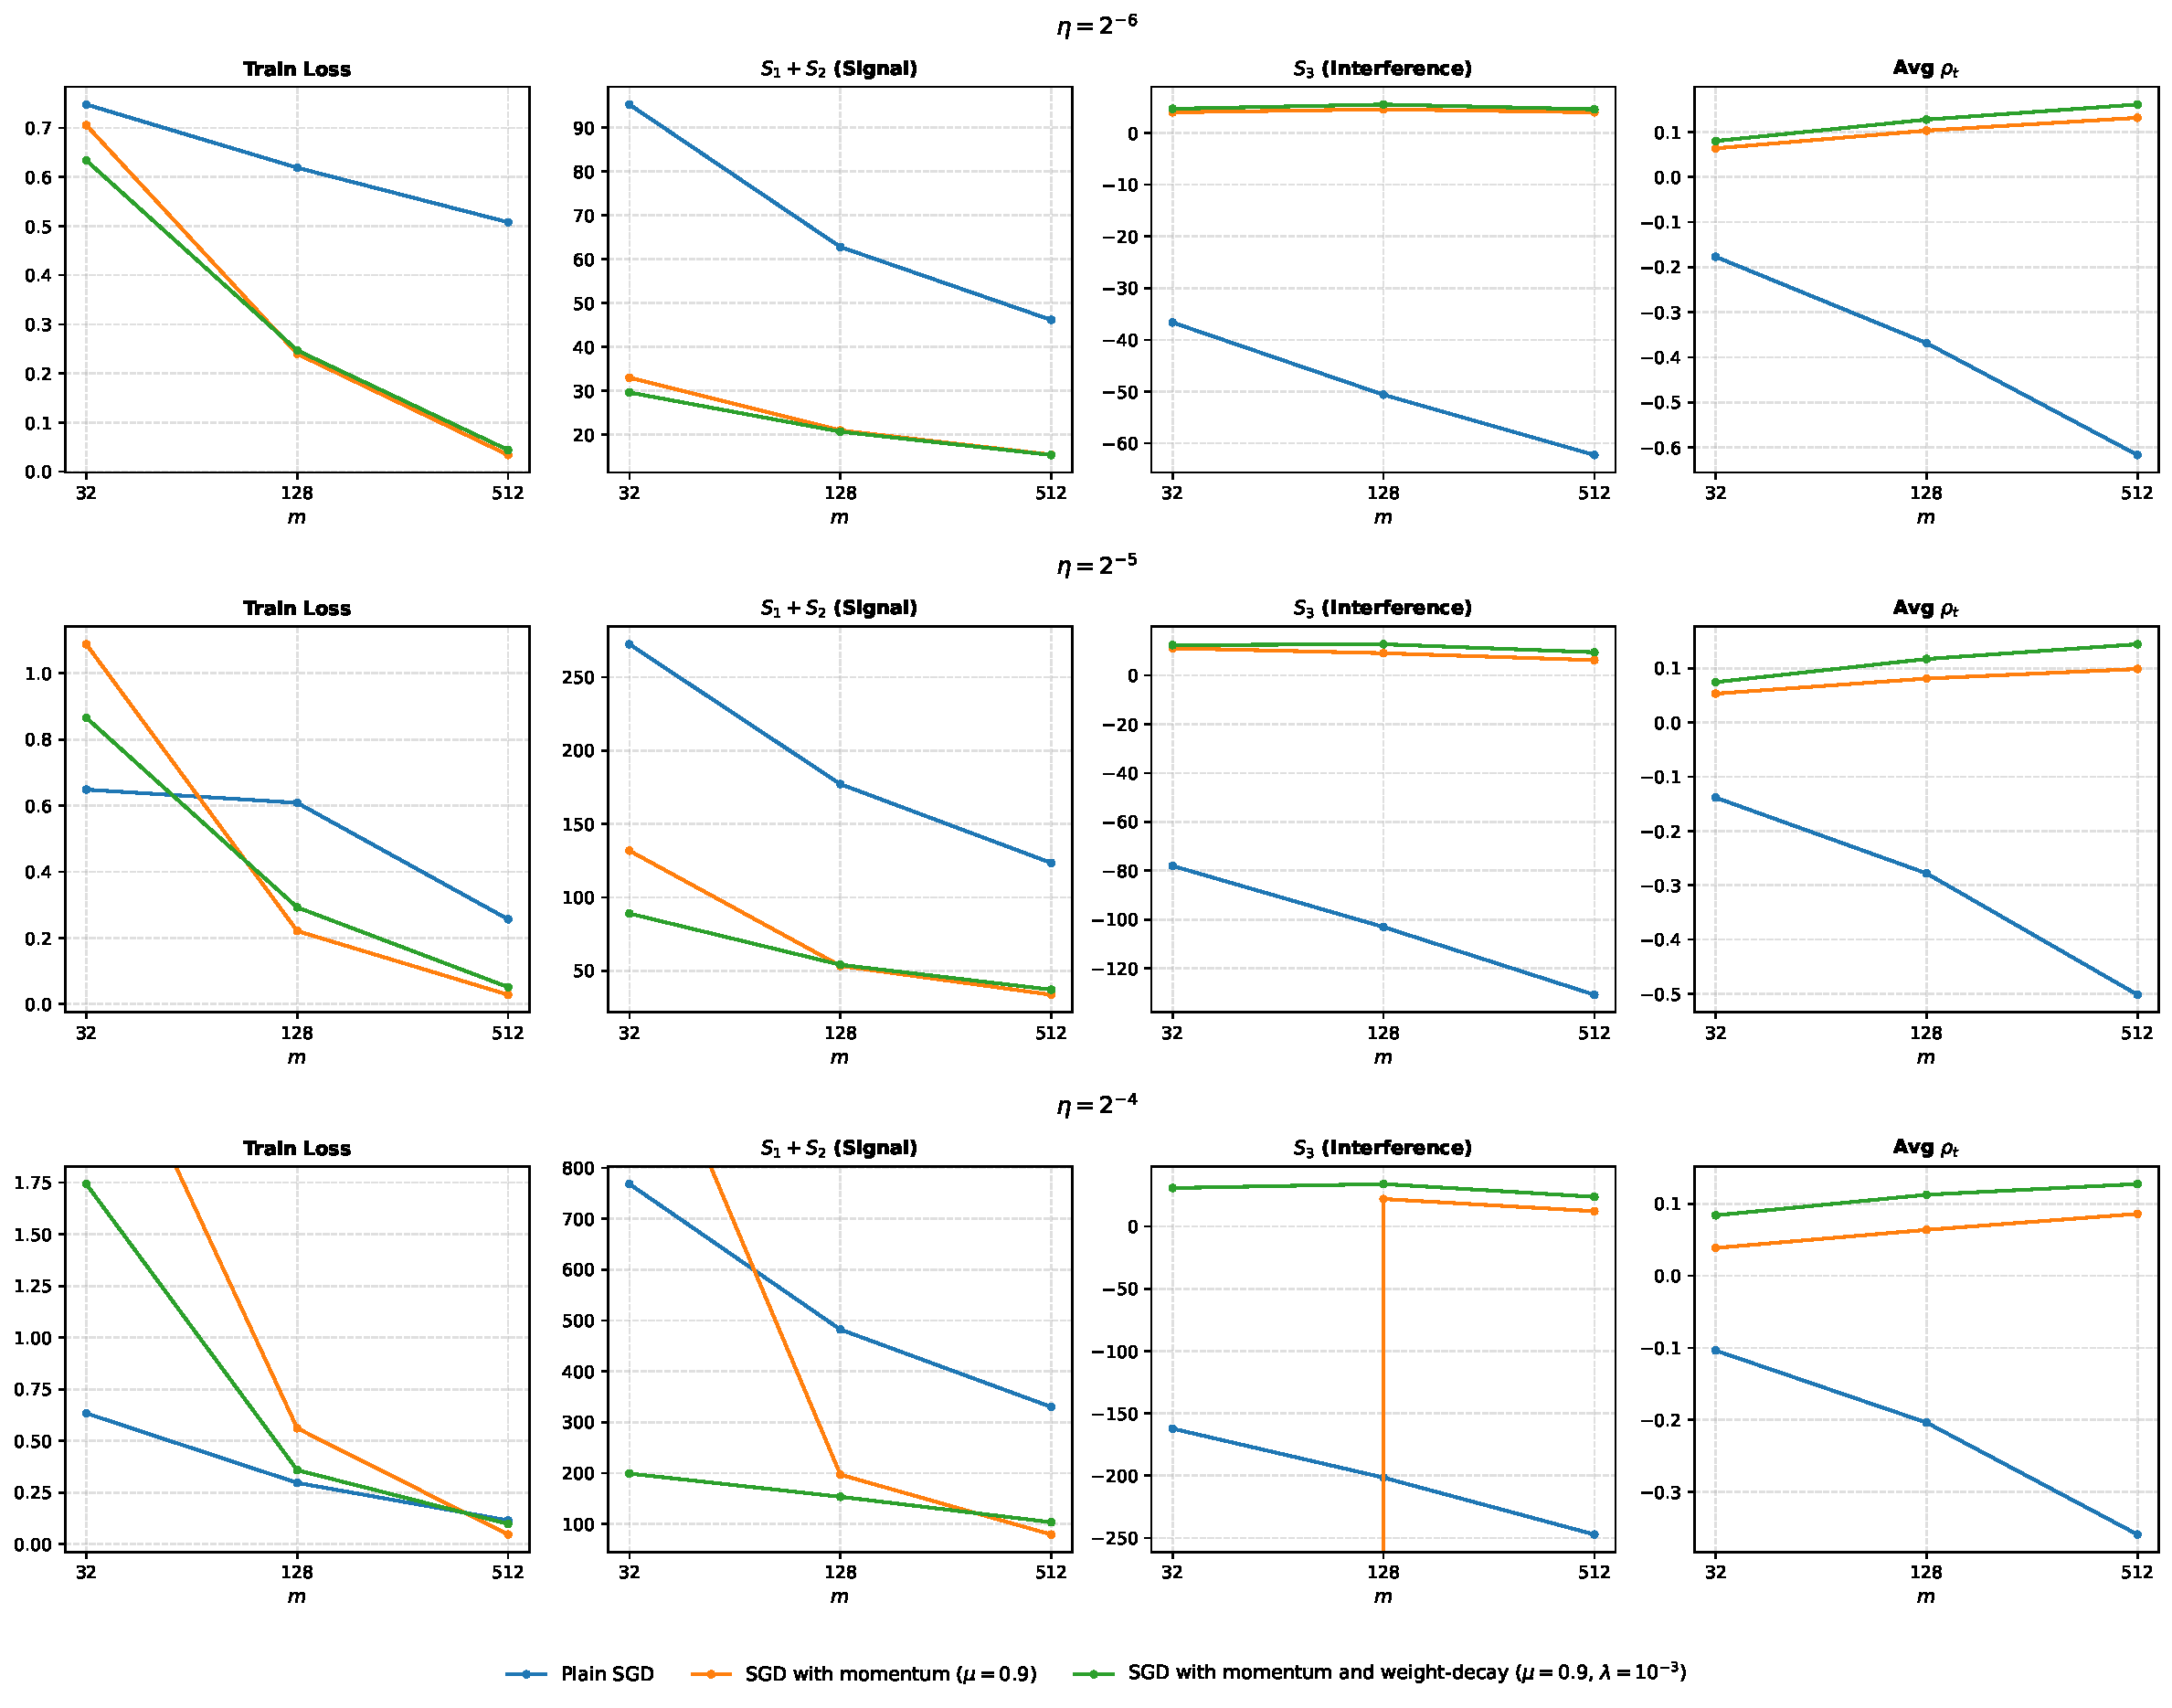
\includegraphics[width=0.95\linewidth]{figures/SGD_ablations_v2.pdf}
    \caption{\textbf{Empirical stability ablations for SGD, momentum, and weight decay.} We sweep batch size $m\in\{32, 128,512\}$ and learning rate $\eta\in\{2^{-6},2^{-5},2^{-4}\}$. Each point corresponds to a run and reports training loss, scaled signal $S_1+S_2$, scaled interference $S_3$, and the average consecutive-gradient cosine similarity $\overline{\rho}_t$.}
    \label{fig:stability_ablations}
\end{figure*}

We complement the preceding trajectory analysis with an aggregated view of stability across hyperparameters. We sweep the batch size over $m\in\{32,128,512\}$ and the learning rate over $\eta\in\{2^{-6},2^{-5},2^{-4}\}$ for plain SGD, SGD with momentum, and SGD with momentum and weight decay. Figure~\ref{fig:stability_ablations} reports the final training loss, the terminal scaled signal $\frac{\eta^2}{m^2}(S_1+S_2)$ and interference terms $\frac{\eta^2}{m^2}S_3$, and the average gradient cosine similarity $\overline{\rho}_t$. Unlike the trajectories discussed earlier, this sweep compares the behavior across methods at matched $(\eta,m)$. A central pattern is that larger batches improve all three methods, but they do so through different combinations of signal and interference.

Plain SGD remains in a destructive cross-step regime throughout the sweep. For every $\eta\in\{2^{-6},2^{-5},2^{-4}\}$ and every $m\in\{32,128,512\}$, the average gradient similarity is negative $(\overline{\rho}_t<0)$ and the corresponding cross-step term is also negative $(S_3<0)$. At a fixed learning rate, decreasing the batch size worsens the loss, increases $S_1+S_2$, and moves both $S_3$ and $\overline{\rho}_t$ toward zero. This shows that $S_1+S_2$ should not be interpreted directly as a more useful signal: it is an update-energy term, and it can grow simply because the gradients become noisier. The sweep suggests that reducing the batch size pushes plain SGD toward a noisy drift regime, whereas increasing it moves SGD toward a more coherent but more strongly interfering regime. Plain SGD thus appears to operate between two unfavorable extremes: random drift at small batch sizes and destructive interference at large batch sizes.

Introducing momentum $(\mu=0.9)$ moves the trajectory into a constructive regime ($\overline{\rho}_t>0$ and $S_3>0$) not seen in plain SGD. For $\eta\in\{2^{-6},2^{-5}\}$, the constructive cross-step coincides with lower loss, especially for $m\in \{128, 512\}$. At the more aggressive learning rate $\eta=2^{-4}$, however, we observe the failure mode of momentum: the loss increases sharply, $S_1+S_2$ grows dramatically, and $S_3$ exhibits an unbounded negative excursion. Increasing the batch size mitigates this effect by making consecutive gradients more coherent, which improves the quality of temporal averaging and restores the low-loss constructive regime. 

Adding weight decay further improves the momentum regime, mainly in the more aggressive settings. Its clearest benefit appears at $\eta=2^{-4}$, where it suppresses the growth of $S_1+S_2$ and avoids the extreme breakdown observed for momentum alone at $m=32$, preserving positive alignment. In this sense, weight decay makes the momentum regime less sensitive to aggressive hyperparameter choices, consistent with the recency-bias interpretation.

%\subsection{Batch Representativeness and Noise}
\subsection{Batch Representativeness and Trajectory Coherence}
\label{subsec:batch-representativeness}


\begin{figure*} [h]
    \centering
    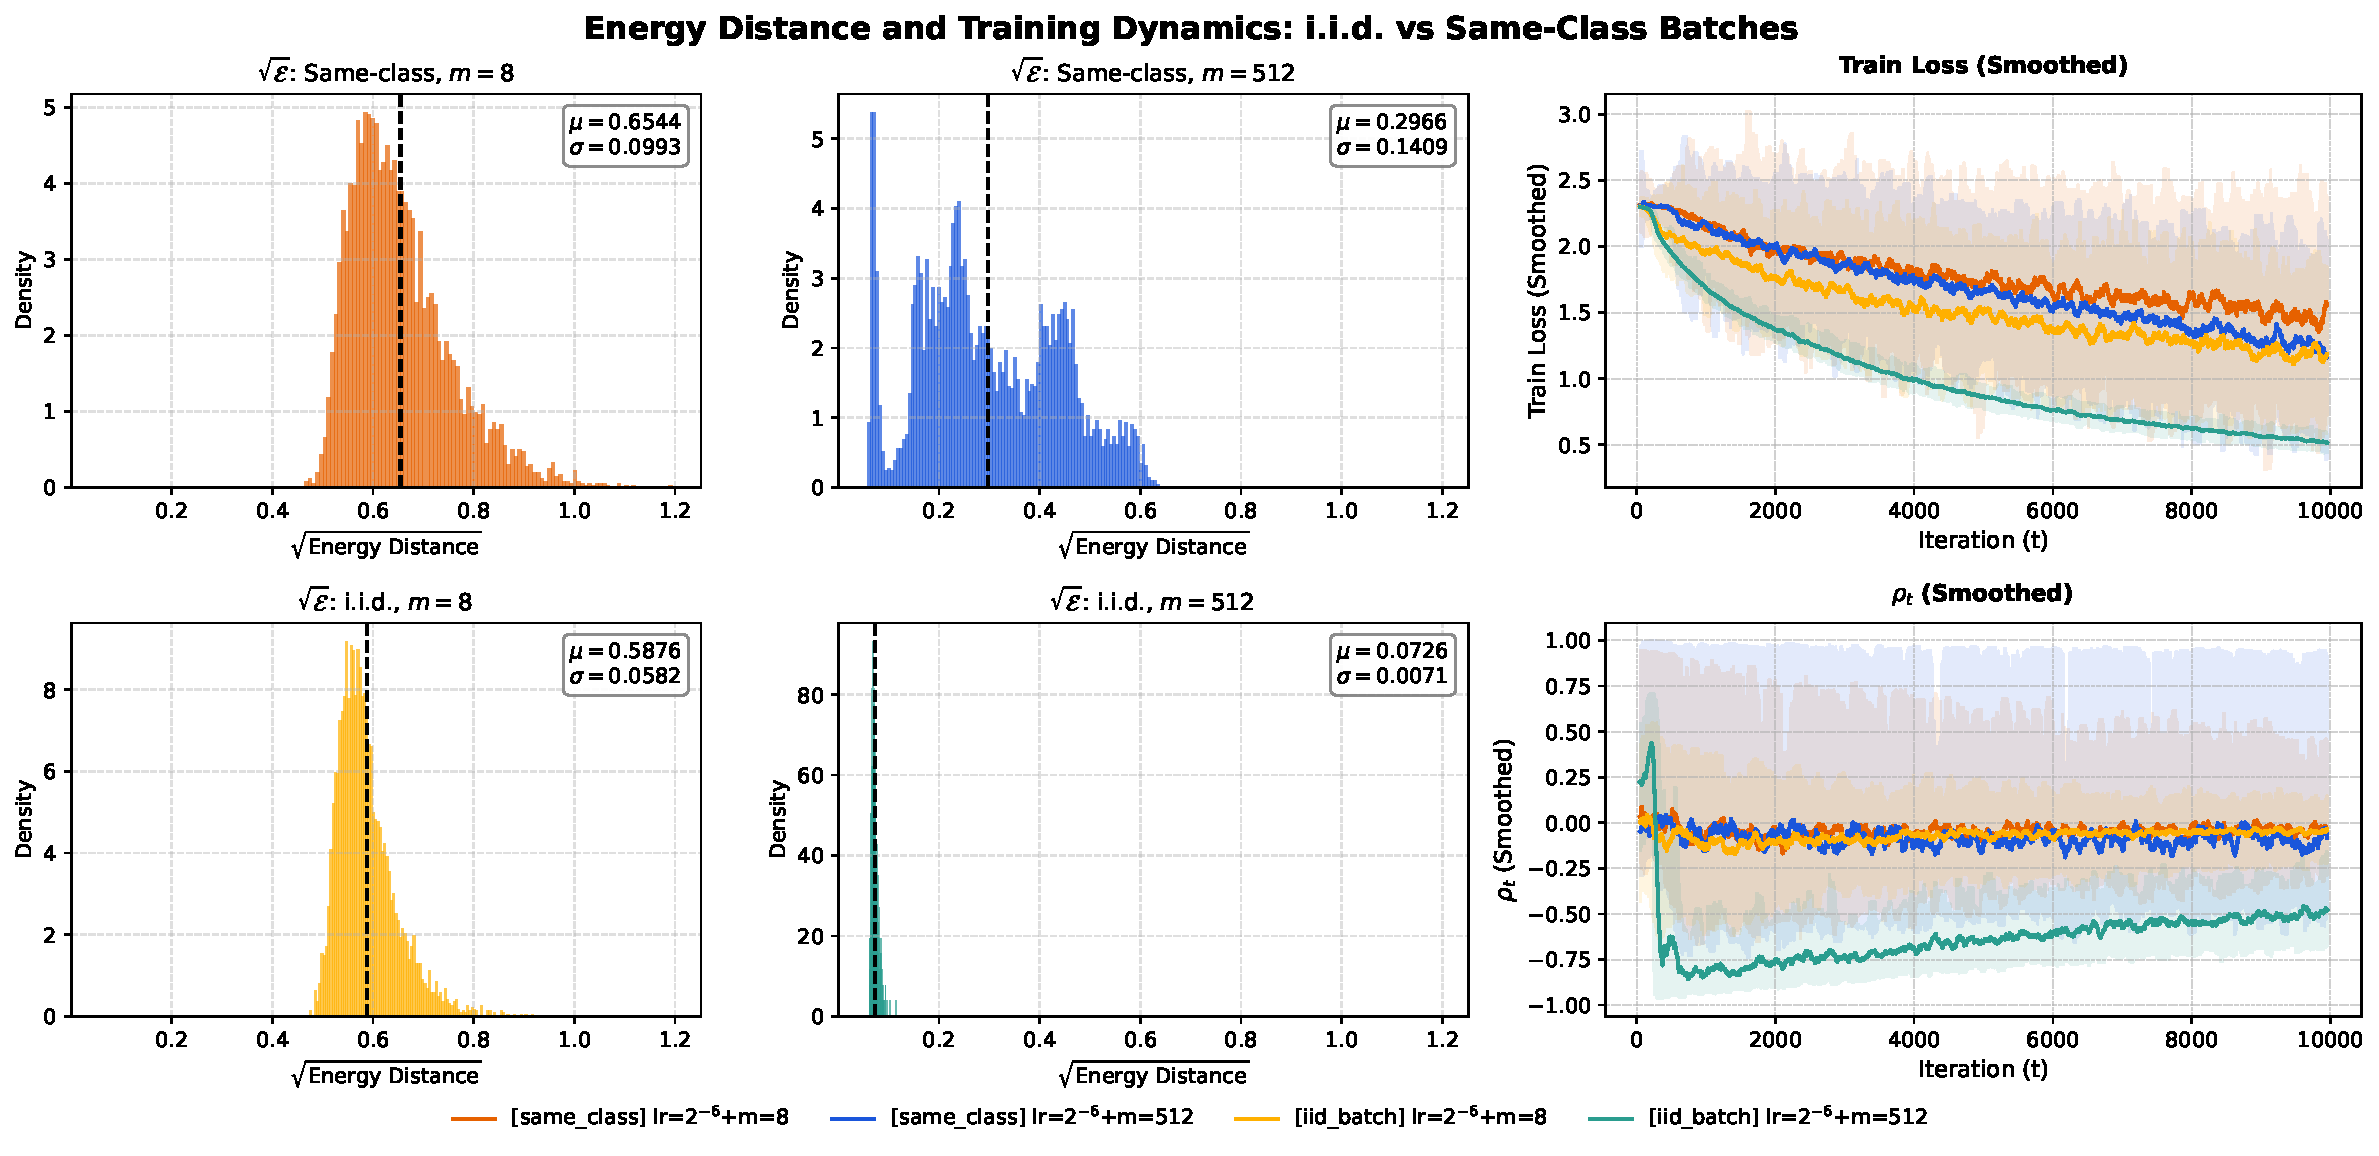
\includegraphics[width=1\linewidth]{figures/combined_energy_training_v2.pdf}
    \caption{\textbf{Effect of batch construction on consecutive-batch energy distance, and noisy trajectories at large batch sizes.} Histograms comparing same-class and i.i.d.\ sampling for $m=8$ and $m=512$. The horizontal axis shows $\sqrt{\mathcal{E}(X_{t-1},X_t)}$ (used to expand the scale for readability). Same-class sampling has a minor effect for $m=8$ ($\mu$: 0.58 $\to$ 0.65) but a large effect for $m=512$ ($\mu$: 0.07 $\to$ 0.29), indicating substantially higher inter-batch discrepancy at large batch sizes. Training loss and $\rho_t$ trajectories: same-class grouping prevents large batches from becoming representative, keeping consecutive updates weakly aligned (small average $\rho_t$) and yielding random-walk-like drift even at $m=512$.}
    \label{fig:energy_distance}
\end{figure*}



The ablations above suggest that training becomes less stable at small batch sizes because the trajectory becomes increasingly random, as indicated by \(\overline{\rho}_t \to 0\) for all cases. Here we argue that this effect is largely driven by limited batch representativeness. Under uniform sampling, each mini-batch \(X_t=\{\mathbf{x}_{t,i}\}_{i=1}^{m}\subset D\) provides only a finite approximation of the training distribution. When \(m\) is small, consecutive batches can differ substantially, leading to larger fluctuations in the gradient direction from one step to the next. As \(m\) increases, each batch becomes more representative of the dataset, and the resulting updates become more consistent across iterations.

Because our experiments use image data, we quantify batch representativeness directly in input space\footnote{For text data, an analogous notion of batch representativeness may be more naturally measured in embedding space, where distances can better reflect semantic similarity than raw token-space comparisons.} by measuring the \emph{energy distance} between consecutive mini-batches~\cite{szekely2013energy}. Given two successive batches, \(X_{t-1}=\{\mathbf{x}_i\}_{i=1}^{m}\) and \(X_t=\{\mathbf{x}_j\}_{j=1}^{m}\), we estimate this distance as
\begin{equation}
\begin{aligned}
\widehat{\mathcal{E}}(X_{t-1},X_t)
&=
\frac{2}{m^2}\sum_{i,j}\|\mathbf{x}_i-\mathbf{x}_j\| \\
&
-
\frac{1}{m(m-1)}\sum_{i\neq i'}\|\mathbf{x}_i-\mathbf{x}_{i'}\| \\
&
-
\frac{1}{m(m-1)}\sum_{j\neq j'}\|\mathbf{x}_j-\mathbf{x}_{j'}\|.
\end{aligned}
\label{eq:energy-sample}
\end{equation}
To effectively control \(\widehat{\mathcal{E}}(X_{t-1},X_t)\), we hold \(m\) fixed and break representativeness on purpose, violating the i.i.d.\ sampling assumption and constructing same-class mini-batches. Our hypothesis is as follows: assuming that batch size improves representativeness (i.e., reduces step-to-step energy distance), then breaking representativeness at a large batch size will reproduce small-batch interference dynamics and worse optimization behavior.
%If batch size helps primarily by improving representativeness (i.e., reducing step-to-step distance energy), then breaking it at a large batch size should reproduce small-batch interference dynamics and worse optimization behavior. 

Figure~\ref{fig:energy_distance} shows that the energy distance distribution between consecutive batches decreases with batch size under i.i.d.\ sampling, while breaking representativeness through same-class batching increases both its mean and variability. This effect is much stronger at \(m=512\) than at \(m=8\), suggesting that very small batches already operate far from the i.i.d.\ regime. The corresponding learning trajectories support this interpretation: when representativeness is disrupted, even large batches recover the noisy, weakly aligned dynamics usually associated with small-batch training. In particular, at fixed \(m=512\), cross-step interference collapses into random drift, and the updates accumulate more like a random walk than a consistent descent direction. These results suggest that much of the batch-size effect is mediated by representativeness: larger batches help because they make successive updates more statistically similar and therefore more temporally coherent. A natural conjecture is that this issue becomes more severe in the scaling regime: as input spaces grow and training data become more diverse, the representativeness of any fixed-size mini-batch should deteriorate, making cross-step coherence harder to maintain and training correspondingly more unstable.




